In this chapter, the mobility in heterogeneous networks will be illustrated via a use case: Electric Vehicle Charging Service (EVCS). There are several reasons for selecting this use case. Firstly, the electric vehicle (EV) is a promising choice for personal transportation in the near future. Secondly, the idea of connecting vehicles is gaining momentum. In addition, a mobile node, an EV in this context, can be connected with the infrastructure via different wireless/wired technologies in different steps (LTE while driving, WLAN while approaching a charging infrastructure, PLC while being docked at a charging infrastructure). Thus, considering multicast in the EV is one step to enable the entertainment system in the EV, which is becoming more and more popular. Moreover, IP multicast can also be used to update the software of the in-vehicle systems.

According to Cisco Internet Business Solutions Group (IBSG) \cite{IBSG_connected_vehicle}, connecting vehicles creates such significant benefits as traffic safety, environmental eco-friendly, easing traffic congestion, and enhancing driver/passenger experience (in-vehicle infotainment systems). Four key capabilities in the connected vehicle are connection within the car, connection to personal devices, connection \textit{around} the car and connection to the cloud (or infrastructure). These capabilities make a vehicle as a \textit{personal digital assistant on wheels} \cite{IBSG_connected_vehicle2} keeping peoples connected to the Internet of Things. Thus, they make our travel experience safer and more convenient as well as enhance the in-vehicle experience \cite{IBSG_connected_vehicle2}. In line with this trend, the EVCS gains the benefits of connecting vehicles to provide a smart charging service from both user and electricity operator perspective. 

\section{Introduction}
The number of vehicles in use is set to increase exponentially in recent years (1.015 billion in 2010 \cite{vehicle_population}). This trend causes some serious issues regarding energy sources like increasing in fuel demand and costs \cite{evci_mit}, environmental concerns \cite{gas_emission} and air quality. On one hand, it encourages the production and use of clean and efficient energy vehicles in which the electric vehicles (including full electric and plug-in hybrid electric vehicles, in common, EVs) belong to. On the other hand, the evolution of battery technology allows increasing the battery capacity while decreasing the weight/size of battery pack and reducing the costs. This context makes the EV a promising choice particularly for individual mobility in the cities.

In order to gain the customer acceptance of the EV, the charging infrastructure needs to be deployed at least as numerous and widespread as the fueling stations. Yet, unlike the fueling station, the various available charging strategies requires unprecedented interactions between drivers and the Grid operators. Secondly, the type of charging stations will range from the commercial stations to the single plugs operated in parking lots or in residential areas. Altogether, this will lead to a segmentation of Electric Vehicle Charging Services (EVCS), with a complex tracing of charging contexts and payment, which would make the charging process difficult and charging capacity/need unforecastable for Grid operators, adding anxiety to users and Grid operators. One solution to mitigate such situation is to make heterogeneous charging strategies and stations, as well as  and the natural mobility of EVs transparent to the EVCS. 

As stated in \cite{EV_smart_grid}, the critical requirement to get energical and economical benefits from Smart-grid and EVs is to reach an optimal scheduling of charging EVs and storing electricity by EV. 
Uncoordinated burst of EV charging may cause a huge energy demand that can result in the electrical grid congestion, while storing electricity by EVs may be inefficient if required immediately elsewhere. Thus, it is important for Grid operators to monitor the necessary data (like energy consumption and demand) and to assign and route vehicles to the appropriate charging stations supporting their required charging policies. Such negotiation cannot be conducted at the charging station but must be conducted while driving. The EV therefore needs to communicate with the charging infrastructure \cite{plc_smart_grid}. In this context, several access technologies (e.g., WLAN, LTE and Power Line Communication (PLC) \cite{wireless_plc}\cite{plc_full}) must be used at different phases of the EVCS, such as LTE while driving, WLAN while approaching a charging station, and PLC while being docked at a charging station. Such heterogeneous communication technologies should be transparent to the user, the Grid operator and to the EVCS in order to maintain the service context. 

In this chapter, we propose an EVCS solution from both user and Grid operator point of view. For the user, it provides a ubiquitous and transparent charging service at different scenarios (at home, at a charging station and at a parking), making charging an EV as simple as possible. It also helps the Grid operator to efficiently manage the user consumption/demand to control the load on the grid especially when a large number of EVs is considered. From the centralized nature of Smart-grid services, a network-based IP mobility management solution, Proxy Mobile IPv6 (PMIPv6) \cite{PMIPv6}, is most appropriate to federate segmented charging services and make the charging experience transparent to EVs mobility as well as the communication technology used by each phase of the EVCS. By using PMIPv6, the service takes care of the EV mobility, handling vertical and horizontal handovers between different communication technologies (e.g., WLAN, LTE and PLC). Yet, IPv6 address preservation in PMIPv6 remains an issue in such context, and we provide a solution by relying on a logical interface approach to hide the change of interface to the IPv6 stack. Finally, we will validate the EVCS concept and the performance of PMIPv6 for the EVCS against benchmark from IEEE 1646. The mobile multicast in heterogeneous networks is also taken into consideration. A near-to-real testbed, which is a combination of real and virtual machines, has been deployed to reduce the hardware cost and to provide more flexible experiment. A real PLC connection provided by partners from the VELCRI project is used to obtain realistic results.\\ 

In the context of this thesis, this chapter discusses the mobility of the nodes in heterogeneous networks, mainly from a mobile node point of view. In other words, the MN will move in a PMIPv6 domain using different access technologies e.g., WLAN, LTE and PLC. Thus, both vertical and horizontal handover will be considered. A vertical handover is executed when the mobile node changes the type of technology it uses to access the network, while a horizontal handover is performed between two layer 3 point of attachment using the same technology. Also, IP multicast will be taken into account. From a mobile node point of view, to obtain the same IPv6 address when switching between different interfaces, logical interface mechanism is used. Moreover, it helps to hide the changing of the interfaces from multicast application point of view. Also, the IEEE, through its 802.21 work group\footnote{IEEE 802.21 Working Group, http://www.ieee802.org/21/index.html}, has developed a standard that allows a MN to seamlessly roam across different types of 802 network access technologies e.g., WLAN, WiMAX and LTE. The solution based on the Media Independent Handover (MIH) Services has been deployed in the Medieval project \cite{d4.1}. Thus, we do not mention MIH-based solution in this chapter. 

The structure of this chapter is as follows. Section \ref{ch8:evcs} describes a solution for EVCS regarding different charging use cases, design principles, and operations. Section \ref{ch8:pmip} briefly introduces PMIPv6 in the context of EVCS and considers multicast in the context of EVCS and heterogeneous networks. While section \ref{ch8:experimentation} describes the testbed, experiment scenarios and the experiment results. Finally, conclusions are presented in the last section.

\section{Electric Vehicle Charging Service} \label{ch8:evcs}
In this section, starting from the deployment scenarios for EVCS, the usage scenarios, the design principles as well as the operations of the EVCS are briefly provided. Further discussions on EVCS can be found in \cite{PMIP_EV,velcri_report}. This section also makes an early highlight on the reasons why PMIPv6 is a good choice in the context of EVCS.

\subsection{Electric Vehicle Charging Deployment}
In the context of VELCRI project, there are three types of charging strategies, namely standard, rapid and ultra-rapid. The standard charge may take from 4 to 8 hours to provide a full charge upon the initial state of battery, while the rapid and the ultra-rapid charge need about 30 minutes and 5 minutes, respectively. The location of the charging pods may vary, however, three typical places with the corresponding characteristics are considered:
\begin{itemize}
\itemsep 0.1em
\item Charge at home: long charging time at low power;
\item Charge at a station: short charging time related to average fueling time; requires a high peak power level, which limits the simultaneously charging pods at stations;
\item Charge at a parking: charging time related to the time spent in the parking, reduced peak power but large amount of charging pods, which requires flexible charge scheduling.
\end{itemize} 

From the characteristics of different types of charge and locations, Table.~\ref{tap:type_location} shows the possible deployment scenarios of charging system. It is worth noting that the scenarios marked $\textit{possible}$ are not considered in this chapter.

\begin{table}[ht]
\footnotesize
\captionsetup{font=footnotesize}
\caption[Electrical vehicle charging system deployment: type and location.]{Charging System Deployment: Type and Location}
\label{tap:type_location}
\centering
\begin{tabular}{|c |c |c |c |}%{|l|l|l|l|l|l|}%
\hline
\textbf{Charge Type $\backslash$ Location} & \textbf{Home} & \textbf{Station} & \textbf{Parking}   \\
\hline
\textbf{Standard charge} &  $\surd$ & - & (possible)\\
\hline
\textbf{Rapid charge}  & - &  (possible)  & $\surd$ \\
\hline
\textbf{Ultra-rapid charge} & - & $\surd$&  (possible)  \\
\hline
\end{tabular}
\end{table}

\subsection{General Use Cases for Electric Vehicle Charging Service}
\begin{figure}[h!] 
 \begin{center} 
 \includegraphics[width=0.75\textwidth]{./Part2/Chapter6/figures/c8_use_cases.eps}
    \caption[General use cases of the electrical vehicle charging service]{General use cases of EVCS.}
     \label{fig:c8_use-cases}
  \end{center} 
\end{figure}

Based on the charging deployment scenario, four general use cases for the EVCS are considered (see Fig.~\ref{fig:c8_use-cases}): (a) charging at home, (b) charging at a station, (c) charging at a parking, and (d) moving between the stations/parkings. 
\paragraph{Charging at Home} The network at home can be considered as home network of the EV. The EV is typically charged in the evening (period of high energy demands and high cost) when the EV owners return home. Thus, the EV needs to be charged intelligently. It can be done thanks to the intelligent charging management which is responsible for the automatic charge/discharge of the EV in order to lower cost and effectively control/optimize the load on the grid.
\paragraph{Charging at a Station} The EV, at first, communicates with the infrastructures via the wireless access technologies e.g., WLAN and LTE to assign and route vehicles to the appropriate stations. At the station, the EV will be plugged into an electrical outlet (using PLC connection) to charge. A vertical handover between WLAN/LTE and PLC will be performed that allows the EV to continue communicating with the charging station. Again, the charging process will be taken care by the intelligent charging management. The EV can also use additional services during the charging process. After the charging is done, the EV may receive a bill including the charging-related information (time and cost), the EV profile and operator's information.  
\paragraph{Charging at a Parking} The steps prior to parking are similar to those in the previous case (charging at a station). The charging schedule can also be negotiated. Because of the difference between station and parking, localized service can be provided to route vehicles to the appropriate charger. 
\paragraph{Moving between the Parkings}
In some cases, the charging process is interrupted. The context related to this EV will be stored at a database. After connecting to another parking, the EV can make an attempt to keep the same negotiation or fall back to a renegotiation in case the parking fails to support the requirements. In the first case, the context will be restored (preservation of the context) at the current parking.
\subsection{Design Principles}
To deal with different usage scenarios of EVCS, we proposed a solution guided by a set of design
principles as follows:
\begin{itemize}
\itemsep 0.07em
%\vspace{-0.07in}
\item Transparency: transparent mobility of the user to the service. It allows EVs to use the charging system as similar as at home (e.g., context preservation and under only one contract);
\item Pre-negotiation: negotiation with the charging infrastructure before deciding to go to a specific station/parking to charge (pre-negotiation);
\item (Intelligent) Charging management: cost minimizing (for user) while maximizing system reliability and stability (for Grid operator);
\end{itemize}

Moreover, the EVCS should provide an easy-to-use service and secured transactions (from user perspective), as well as an effective way to manage the user information (energy demand, consumption, and location) to better control the load on the grid (from Grid operator perspective).

Therefore, the charging service can be divided into the basic modules which are mapped to the design principles as described in Fig.~\ref{fig:modules}.
\begin{figure}[h!] 
 \begin{center} 
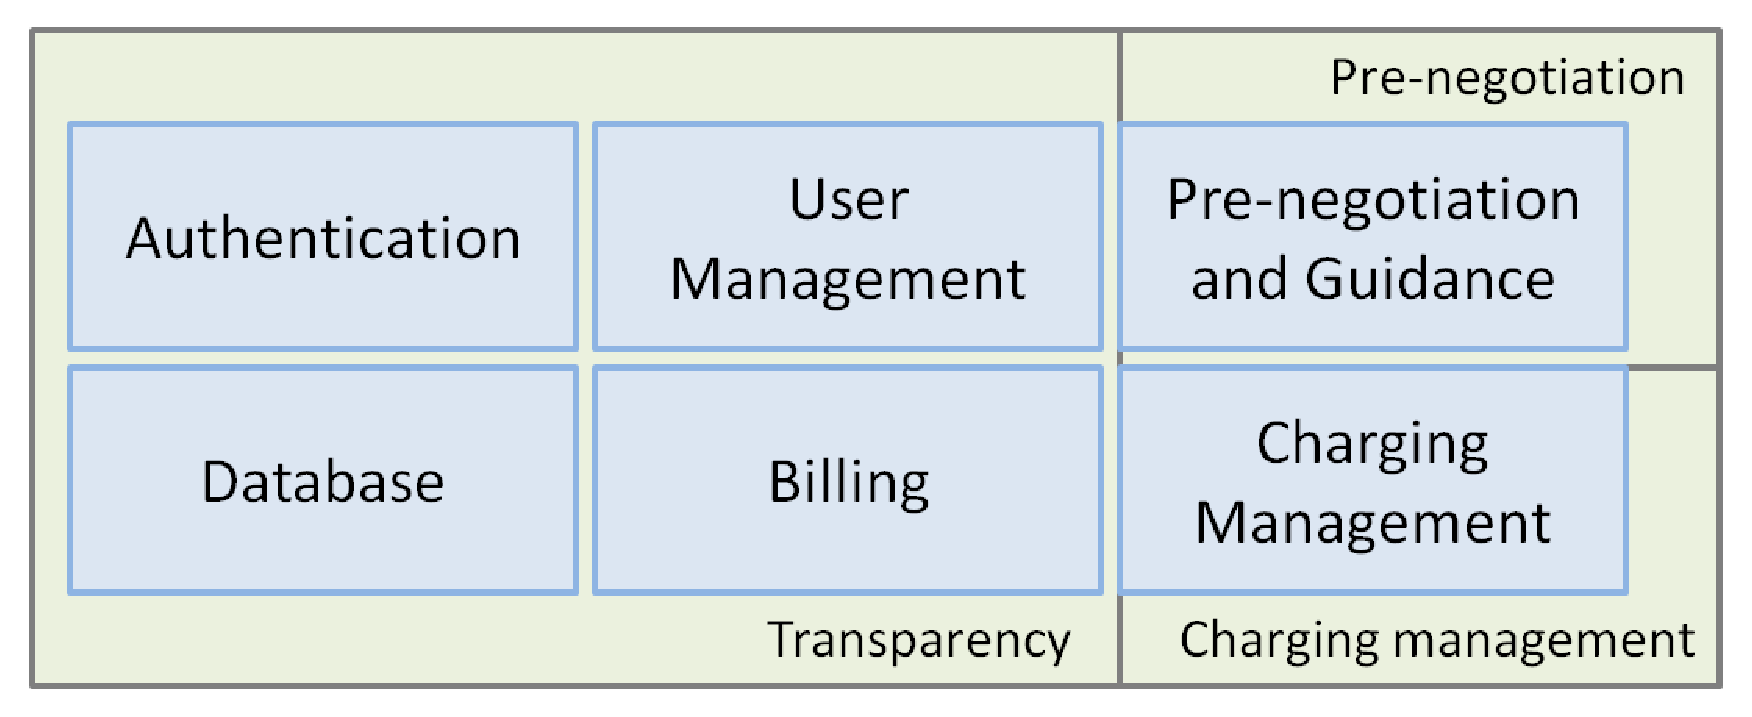
\includegraphics[width=0.6\textwidth]{./Part2/Chapter6/figures/modules.eps} 
   \caption[The EVCS's modules.]{EVCS modules reflect the design principles.}
   \label{fig:modules}
 \end{center} 
\end{figure} 
\subsection{EVCS: Operations and Functionalities}
Following its design principles, the EVCS is proposed with the main operations as briefly described as follows (further information can be found at \cite{velcri_report}):
\paragraph{Session initiation (via WLAN/LTE/PLC)} It is executed when an EV is connected to the charging infrastructure for authenticating/authorizing and obtaining the EV profile (context establishment). PLC is used for the session initiation only in case of charging at home. 
\paragraph{Session negotiation and guidance (via WLAN/LTE)} This operation allows the EV to negotiate with one or multiple charging infrastructures to find the most appropriate one based on such metrics as charging time, cost (for user), charging type, required capacity and slots availability (for Grid operator). It is noted that this step is executed before reaching a charging station/parking thanks to the wireless access technology (WLAN/LTE). Also, additional information of the station/parking can be provided like discounts and bonuses.
\paragraph{Charging management (via PLC)} Charging process does not start as soon as the EV is plugged, but is rather scheduled according to the capacity of the grid and the demand of the user established during the negotiation phase. Accordingly, an intelligent charging management unit coordinates the charging process on bi-directional communication link between the infrastructure and the EV while being plugged. In other words, the EV can be charged when the demand is low, otherwise it can be considered as a distributed energy source when the demand is high.  
\paragraph{Session termination (Billing, via WLAN/LTE/PLC)} When a session is terminated, electricity used or sold as well as related statistics (price, charging time and charging type, etc.) will be logged to the service provider and the cost charged on the user account as if the user was at home. 

\section{PMIPv6 for Electric Vehicle Charging Service} \label{ch8:pmip}
In the context of EVCS, since an EV can be charged at different places as similar as at home, PMIPv6 is a good choice. It is because it makes heterogeneous communication technologies transparent to the EVCS and hides the mobility of the EVs to the service. 

As we can see in Fig.~\ref{fig:c8_use-cases}, using PMIPv6 offers some benefits in the context of EVCS: (1) Network-based mobility management and Address preservation: The MAG where the EV is currently connected simulates the EV's home network. Therefore, the EV uses the same IPv6 address when moving in a PMIPv6 domain. So, the EV is not aware of the mobility; (2) Context preservation: This feature facilitates the charging process of the EV in case of mobility; (3) Location management; (4) Easy-to-integrate with Authentication, Authorization and Accounting (AAA) mechanism; and (5) EV-Grid interaction: The PMIP messages can be extended for collecting the EV-related information. Thanks to the advantages of PMIPv6, the energy and utility suppliers can provide an easy way but flexible to access their services. 

Although PMIPv6 can bring benefits to the EVCS, it has several limitations. Thus, improvements are needed to make PMIPv6 suitable for the EVCS.
\paragraph{Handover across heterogeneous access technologies (WLAN, LTE and PLC) - IPv6 Address Preservation} Considering handover across different access technologies (vertical handover), there are several mechanisms which allow the EV to obtain the same IPv6 address after handover. The first one is based on the auto-configuration mechanism by using a common identification for both PLC and WLAN interface (like Network Access Identifier). The second one uses the Dynamic Host Configuration Protocol (DHCP) mechanism in which two interfaces must be set with the same client identifier. However, the major limitation of these two approaches is that two interfaces cannot be active at the same time. As the result, it may cause a significant service disruption and packet loss. 
    
The third mechanism uses the logical interface technique \cite{logical_inteface} which allows to hide the different access technologies (e.g., using Linux bridge mechanism). Thus, the changing of interface is transparent to the IP stack. Moreover, two interfaces can be active at the same time. For this reason, this mechanism is more suitable than the others to facilitate the vertical handover in terms of handover latency. Note that in the context of electric vehicle, with a huge power, the impact of power consumption caused by turning on both of the interfaces is negligible. 
\paragraph{Context Preservation} To support the context preservation characteristic, the MN's context needs to be stored in a database/policy profile. One possible solution is that the AAA server is extended to store this type of information. 

\subsection{Multicast Considerations}
\begin{figure}[h!] 
  \begin{center} 
    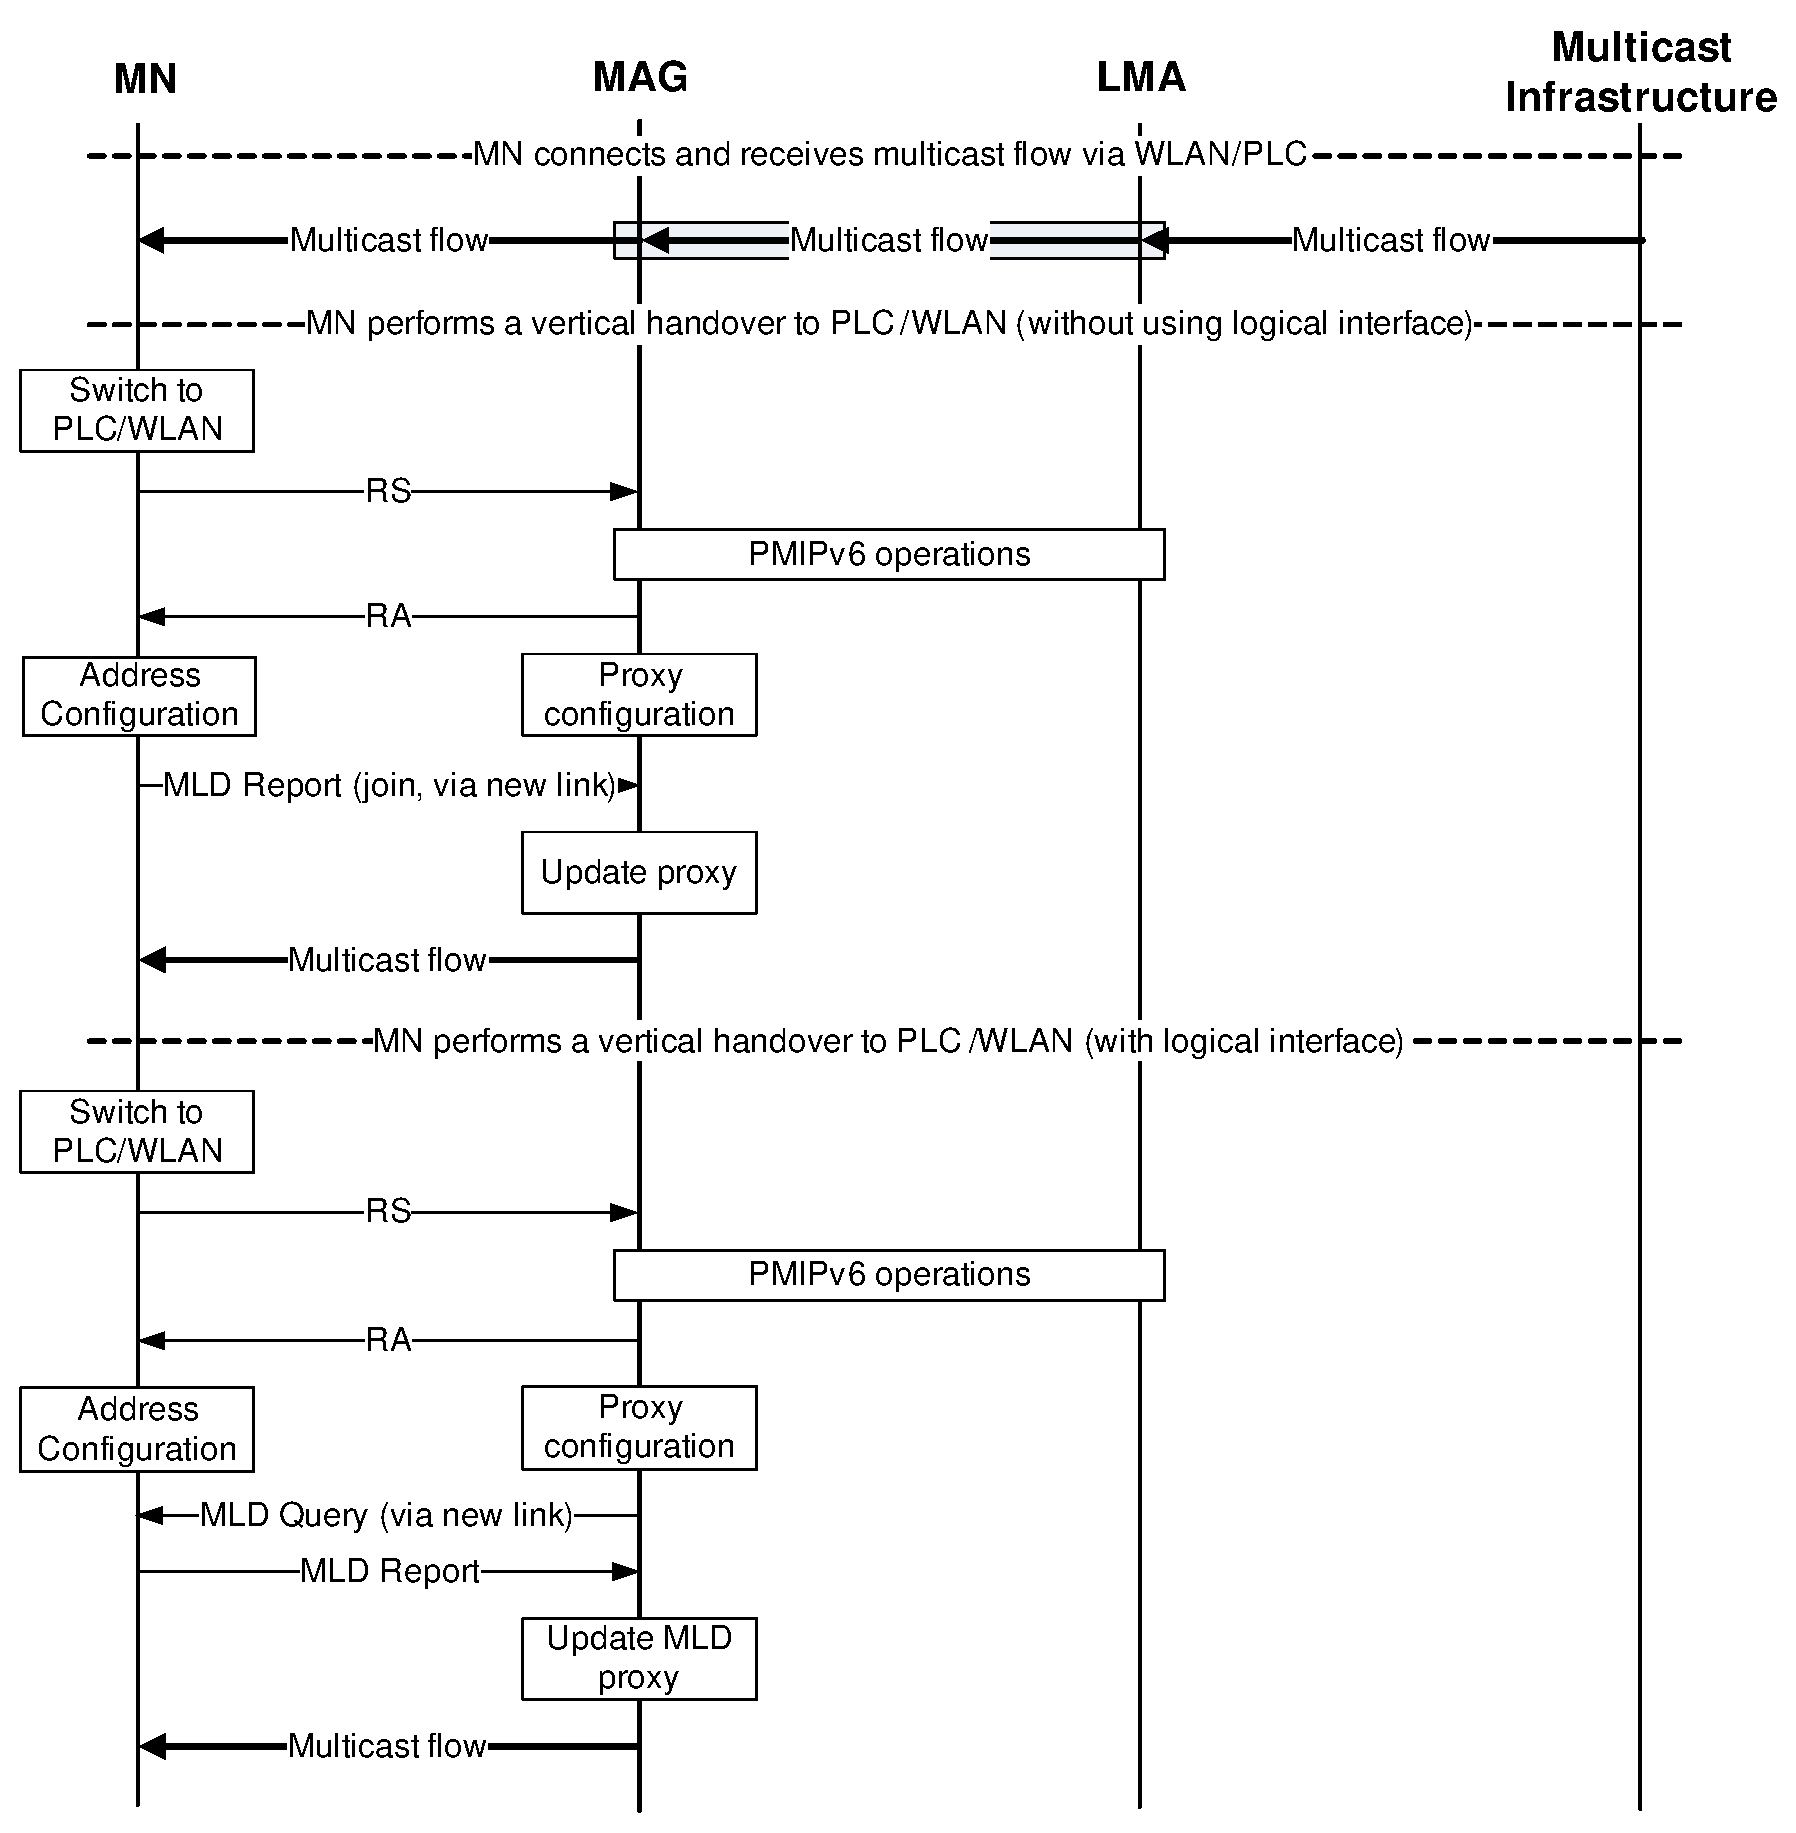
\includegraphics[width=0.80\textwidth]{./Part2/Chapter6/figures/c8_handover_base.eps} 
    \caption[The multicast-related signaling when an EV changes its point of attachment.]{Handover signaling regarding multicast.}
    \label{fig:c8_handover_base}
  \end{center} 
\end{figure}
When an MN (a listener) performs a vertical handover between two interfaces while connecting to the same MAG, the normal PMIPv6 will be executed to allocate a HNP for the new interface. Depending on the PMIPv6 implementation, the MN can obtain the same HNP as for the previous interface or a new HNP. It then configures its IPv6 address based on the prefix allocated. As a normal proxy operation, the MLD proxy at MAG will add the MN to a downstream interface. Moreover, from a listener point of view, the listener should join the on-going multicast flows at the new interface. Thus, the requirement in terms of mobility transparency cannot be guaranteed. Thanks to the logical interface mechanism, the listener does not need to re-join the on-going flows, since the logical interface has already joined them. As a result, the listener is unaware of mobility from the multicast service point of view (see Fig.~\ref{fig:c8_handover_base}). However, even with logical interface, if the on-going flows are not present at this downstream interface, the MN has to wait to receive an MLD Query message to express its active multicast flows by mean of MLD Current State. As stated in the previous section, it may experience a noticeable service disruption (see Fig.~\ref{fig:c8_handover_base}). Thus, the MAG will inform the MLD proxy so that the proxy can update its membership state to forward the on-going multicast flows in the new downstream interface as soon as possible. It can be considered as an extension to MLD proxy. In case of a vertical handover between two different MAGs, the context transfer is needed to reduce the service disruption time as discussed in Chapter \ref{ch:multicast_PMIP}. Again, by applying the logical interface mechanism, the mobility is transparent to the listener.  

When the MN performs a horizontal handover between two MAGs, similarly, the context transfer between these MAGs is required in order to avoid a large service disruption and packet loss. Further information on the handover signaling and operation can be found in Chapter \ref{ch:multicast_PMIP}.
 
\section{Experimentation} \label{ch8:experimentation}
\subsection{Experimentation Setup and Scenarios Description}
In order to validate the proposed solution, a near-to-real testbed has been deployed. In this section, the testbed and the experiment scenarios are presented.
\begin{figure}[h!]
\centering
\subfloat[]{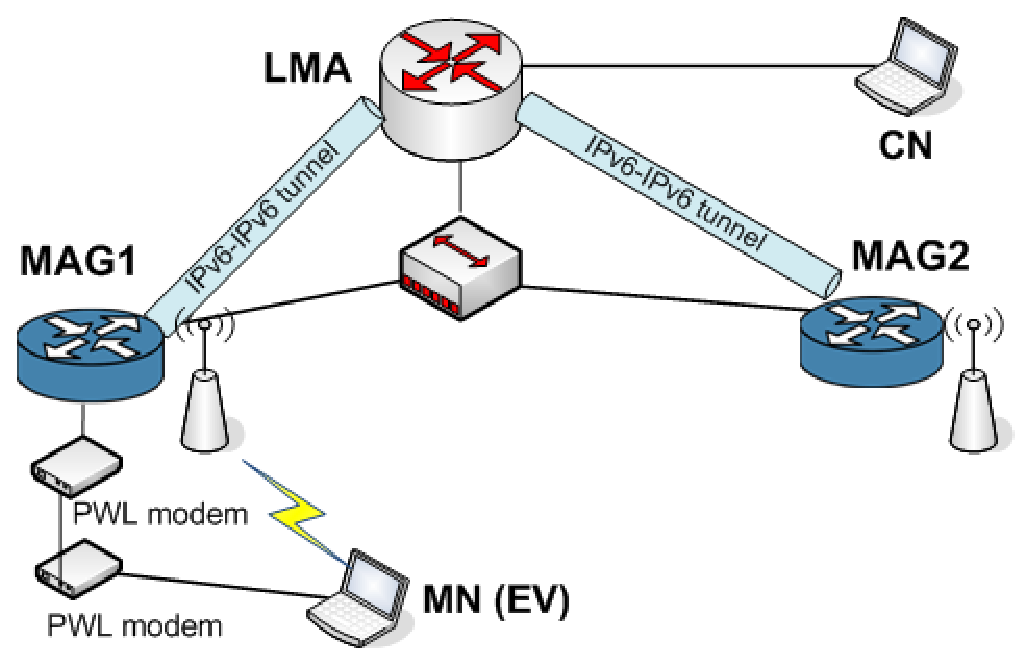
\includegraphics[width=0.47\textwidth]{./Part2/Chapter6/figures/c8_testbed.eps} \label{fig:c8_test-bed}}\,\,\,\,\,\,
\subfloat[]{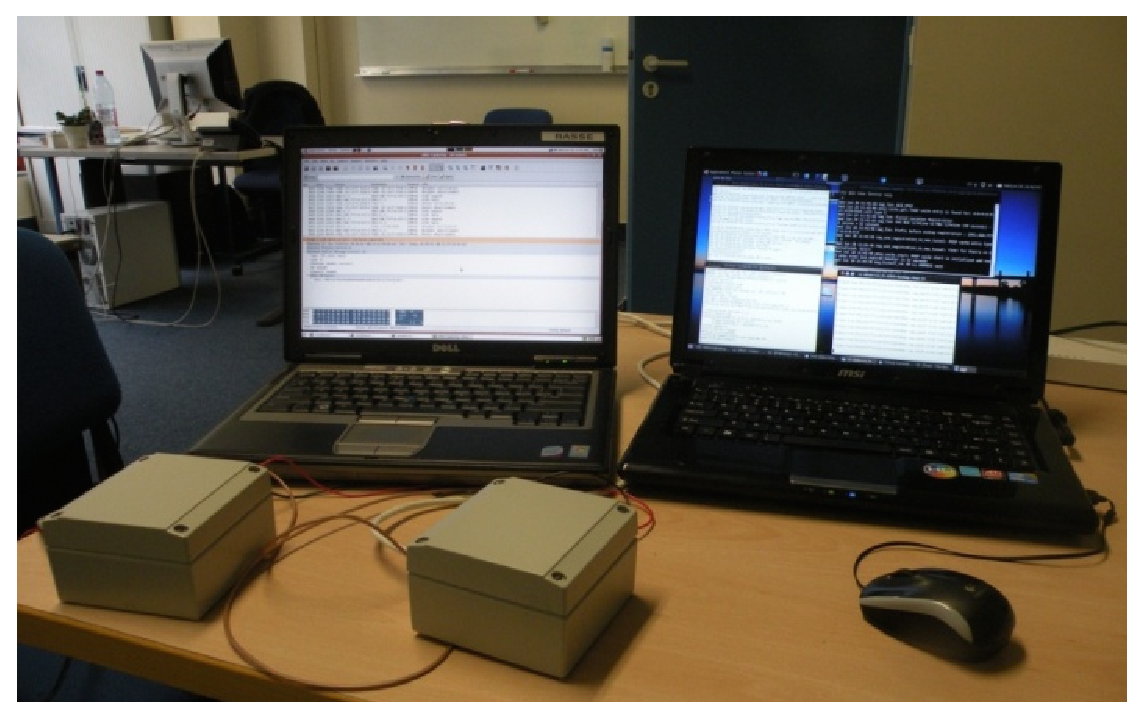
\includegraphics[width=0.47\textwidth]{./Part2/Chapter6/figures/c8_testbed_2.eps}\label{fig:c8_test-bed_2}}
\caption[Testbed implementation for the ECVS experimentation.]{Testbed: a) architecture; b) actual image.}
\label{fig:c8_testbed}
\end{figure}

\paragraph{Description of the Testbed}
The testbed, as indicated in Fig.~\ref{fig:c8_test-bed}, is composed of one LMA, two MAGs, one CN and one MN playing the role of an EV. It is noted that the CN represents an entity in the Smart Grid. The testbed is based on the User-mode Linux (UML) to create the virtual machines. The LMA, the MAGs and the CN are the virtual machines (UML) running on a host machine. Another real machine is used as an EV that connects with the MAG via a WLAN or a PLC connection. To connect the virtual machines, the virtual Ethernet connection is simulated by using a combination of Linux Bridge and TAP interface (for more details, see Chapter \ref{ch:performance_evaluation}). In case of PLC connection, two PLC modems are connected via coaxial cable and to the MN and to the MAG, respectively. Thanks to VELCRI project, a real PLC connection is used in the testbed. The PMIP functionality and multicast support can be deployed similar to in the Chapter \ref{ch:multicast_PMIP}. The actual image of the testbed is described in Fig.~\ref{fig:c8_test-bed_2}. In addition, the mapping between the actual image and the logical components of the testbed is illustrated in Fig.~\ref{fig:c8_mapping}.
\begin{figure}[h!] 
  \begin{center} 
    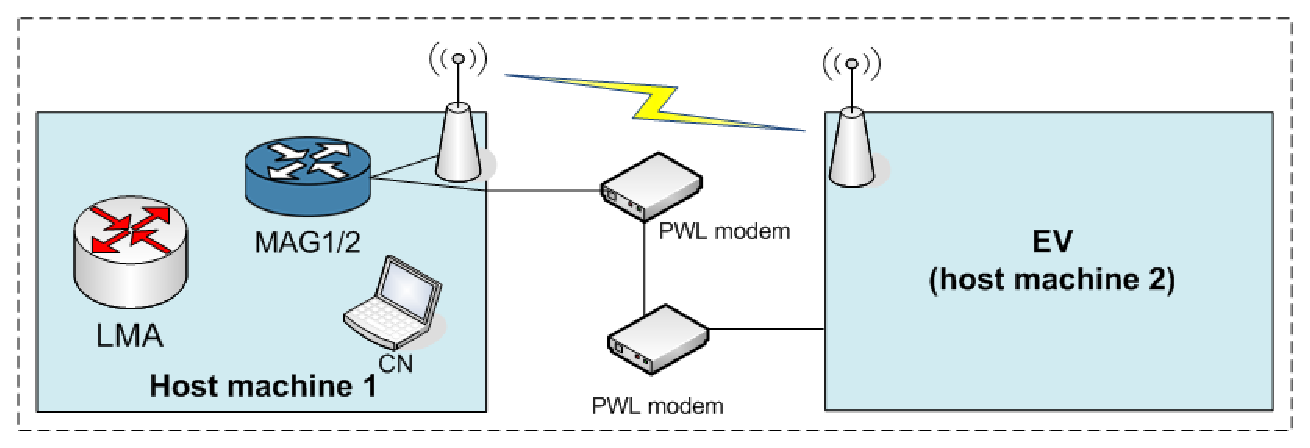
\includegraphics[width=0.65\textwidth]{./Part2/Chapter6/figures/c8_mapping.eps} 
    \caption[Mapping between the actual image and the testbed components.]{Mapping between the actual image and the testbed components.}
    \label{fig:c8_mapping}
  \end{center} 
\end{figure}

During the experiments, a network analyzer tool (e.g., Wireshark) is used to capture the packets exchanged between the entities while a network testing tool (like Iperf) to measure the throughput of WLAN/PLC connection. The Ping application plays the role of a simple service running on EV and CN. When considering multicast, the CN also plays the role of a multicast source broadcasting a multicast flow which is subscribed by the EV (playing the role of a listener).
%\vspace{-0.29in}
\paragraph{Logical Interface Mechanism in Linux}
Logical interface mechanism is applied on the MN using the bridge-utils (bridging)\footnote{Linux Bridge: http://www.linuxfoundation.org/collaborate/workgroups/networking/bridge} and TUN/TAP device for Linux systems as specified in Fig.~\ref{fig:c8_logical_interface}. The TAP device works at the Ethernet frame level while the TUN device acts as a network layer device. We then use the \textit{ebtables} tool\footnote{ebtables – Linux Ethernet bridge firewalling: http://ebtables.sourceforge.net}(or \textit{iptables}\footnote{iptables: http://ipset.netfilter.org/iptables.man.html}), which is a filtering tool for a Linux-based bridging firewall, to switch between the interfaces. 

\begin{figure}[h!] 
  \begin{center} 
    \includegraphics[width=0.4\textwidth]{./Part2/Chapter6/figures/c8_logical_interface.eps} 
    \caption{Logical interface mechanism under Linux.}
    \label{fig:c8_logical_interface}
  \end{center} 
\end{figure}

\paragraph{Experiment Scenarios}
We define four experiment scenarios based on the use cases given in the previous section as follows:
\begin{itemize}
\itemsep 0.07em
\item Scenario 1: Authentication and context establishment. This scenario aims at demonstrating that PMIPv6 can work correctly with PLC.
\item Scenario 2: Vertical handover between WLAN and PLC at one MAG. This scenario describes the transition between the negotiation, the charging management and the termination step. 
\item Scenario 3: (Horizontal) Handover/roaming between two MAGs. From the EVCS point of view, this scenario represents the mobility of the EV between the parkings. It is noted that the horizontal handover in some cases can be replaced by successive vertical/horizontal handovers. Without loss of generality, only a horizontal handover using WLAN is considered.         
\item Scenario 4: Multicast considerations in the scenario 2 and 3. In this case, the CN plays the role of a multicast source broadcasting a multicast flow while the EV plays the role of a multicast listener. Further information about how to generate the multicast traffic in this testbed can be found in Chapter \ref{ch:LB}. In case of handover between two MAGs, the multicast context transfer and the explicit tracking functions are enabled at MAG to reduce the service disruption time as similar in Chapter \ref{ch:multicast_PMIP}.
\end{itemize}

\subsection{Experiment Results and Discussions}
At this step, the experiment focuses on the validation of the concept of EVCS, the performance of PMIPv6 for the future EVCS as well as multicast mobility with heterogeneous communication technologies e.g., WLAN, LTE and PLC. Thus, two evaluation metrics are concentrated, i.e., PMIP functionality and performance metrics which are translated into the corresponding EVCS ones. The first metric aims at validating the functionality of the EVCS regarding the authentication, the context establishment, the address preservation and the service continuity in case of handover. The second metric takes into account the response time (Round-Trip Time (RTT) between the EV and the CN), handover latency, throughput and packet loss in case of unicast traffic; while handover latency, packet loss in case of multicast traffic. From the EVCS point of view, the response time is the time needed for exchanging information between EV and charging infrastructure (stations and Smart Grid) for controlling and monitoring purpose. Handover latency is translated into the time needed to acquisition of the context (IPv6 address) when switching between the operations (negotiation/charging management/termination) in the scenario 2 and when performing handover/roaming between stations in the scenario 3. From multicast service point of view, the multicast service disruption time and packet loss are considered metrics. 

\paragraph{Functionality Metric}
When an EV was connected to a MAG via the PLC connection, the regular PMIPv6 procedures were executed (performing AAA procedures, exchanging PBU/PBA messages, updating binding state at LMA/MAG) to allocate a HNP (2001:100:7777::/64) to the EV. Based on this HNP, the EV configured its IPv6 address (2001:100:7777:021f:3cff:fe59:95a4/64) and used this address to communicate with the CN (scenario 1).

When the EV performed a vertical and a horizontal handover, the EV got the same prefix and kept using the same IPv6 address. By analyzing the packet exchanged between the entities, we can observe that after handover, the EV/CN continues to receive the Echo Request/Reply messages from the CN/EV. From the service point of view, that means the service continues to run after handover.   
%\vspace{-0.13in}
\paragraph{Performance Metric}
The average RTT between the EV and the CN via WLAN connection is 1.98ms (standard deviation ($\sigma$) = 1.47) while via PLC is 3.34ms ($\sigma$ = 0.47). Thus, the values satisfy the timing requirement for monitoring and control information by IEEE 1646 (16ms) \cite{communication_smartgrid}. We can see that although the average RTT in case of WLAN is smaller than that of PLC, the standard deviation in case of WLAN is much higher than the case of PLC. That means the PLC, as a wired link, can provide more reliable connection than the WLAN. Concerning the 
throughput, it is about 4.6Mpbs by using PLC. This value is adequate for the normal traffic services.
 
Regarding handover latency in the scenario 2, since the PLC and WLAN interfaces are activated at the same time, the handover delay is slightly increased compared to the time needed to update the EV location (between the RS and RA message). This value in the experiment is 30ms ($\sigma$ = 10.7) for the handover from PLC to WLAN and 42ms ($\sigma$=12.4) for the handover from WLAN to PLC. In both cases, there is no packet loss. 

In the scenario 3, handover latency is about 2030ms ($\sigma$ = 229.1). This value is much greater than that in the scenario 2. It is due to the time needed to change the mapping of the WLAN interface of the real machine 1 from MAG1 to MAG2 and the time for the tunnel establishment between MAG2 and LMA. This duration in our experiment is quite large (1977ms and $\sigma$ = 242.4).

Based on the handover latency, a threshold value can be defined (e.g., 500 ms) to help the system make an appropriate behavior. For instance, if the handover latency is less than the threshold value, it can be considered as a vertical handover between two interfaces at the same MAG (scenario 2). Vice versa, it can be considered as a handover between MAGs. In the latter case, the session information needs to be stored into the profile server. Yet, some experiments are required to select the most appropriate threshold value.
\paragraph{Multicast Considerations}
When the EV performs a vertical handover from PLC to WLAN at one MAG, the multicast service disruption duration is 53.2ms ($\sigma$ = 23.4). In case of handover from WLAN to PLC, the multicast service disruption time is 70.4ms ($\sigma$ = 21.3). This time consists of the time needed for the typical PMIPv6 operations, the MLD proxy update time and the time for the first multicast packet reaches the MN after handover. 

Similarly, the multicast service disruption time in case of horizontal handover between MAG1 and MAG2 using WLAN is 2038.2ms ($\sigma$ = 332.3). Again, this value is high since the time needed for the switching interface process between MAG1 and MAG2 is large. In this context, we focus on the duration, which mainly consists of the time for the layer 2 handover, the typical PMIPv6 operations, and the multicast-related procedures, which is 176.3ms ($\sigma$ = 63.2). With this value, the handover impact on the quality of multicast stream is almost imperceptible. 

\section{Conclusion} \label{ch8:conclusion}
Using EVCS as a use-case, this chapter discusses the mobility in heterogeneous networks. The consideration of EV's mobility as well as IP multicast in heterogeneous network can be seen as a step towards the era of connecting vehicles.  
From the EVCS point of view, this chapter proposes a solution taking into account different use case scenarios. A centralized IP mobility management solution, PMIPv6, is used to deal with the natural mobility characteristics of the EV. PMIPv6 can facilitate the usage of charging service by keeping the mobility transparent to the user and the Grid operator. Moreover, from a Grid operator perspective PMIPv6 helps to effectively manage a huge number of EVs and to collect the required information of the EV for the Vehicle-to-Grid (V2G) and Grid-to-Vehicle (G2V) purpose. From the multicast service point of view, this chapter investigates the mobility of a listener in heterogeneous networks. Different access technologies are considered as WLAN, LTE and PLC. Both vertical and horizontal handover are taken into consideration. The logical interface mechanism helps to hide the handover between different interfaces as well as to avoid packet loss. Also, the listener remains unaware of mobility from the multicast application point of view, thanks to this mechanism. 

A testbed has been deployed based on the virtual mechanism that allows achieving the near-to-real results at a low cost. In addition, a real PLC connection is used in the experimentation to obtain the realistic results. At this step, from service perspective, the experiment results validated the solution in terms of functionality as well as performance. 

As future work, the EVCS modules will be developed. The (complete) service then will be evaluated in terms of its operations, functionality and performance with different use case scenarios. In addition, we will study the benefits of EVCS in a DMM environment. 



